\paragraph{QuizziPedia::Front-End::Directives::StatisticsDirective}

\label{QuizziPedia::Front-End::Directives::StatisticsDirective}

\begin{figure}[h]
	\centering
	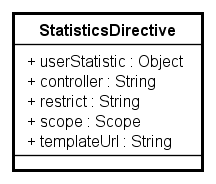
\includegraphics[scale=0.80,keepaspectratio]{UML/Classi/Front-End/QuizziPedia_Front-end_Directives_StatisticsDirective.png}
	\caption{QuizziPedia::Front-End::Directives::StatisticsDirective}
\end{figure}

\begin{itemize}
	\item \textbf{Descrizione}: directive che permette di visualizzare le statistiche di un utente;
	\item \textbf{Utilizzo}: viene utilizzata per mostrare le statistiche nella pagina della visualizzazione del profilo e nella pagina di un utente ricercato;
	\item \textbf{Relazioni con altre classi}:
	\begin{itemize}
		\item \textit{IN} \texttt{UserView}: view contenente i dati personali dell'utente, le sue statistiche relative ai questionari e agli allenamenti effettuati e i questionari a cui è iscritto;
		\item \textit{IN} \texttt{OtherUserView}: view contenente i dati personali e le statistiche di un utente ricercato;
		\item \textit{IN} \texttt{StatisticsController}: questa classe permette di le statistiche di un utente;
		\item \textit{IN} \texttt{StatisticsModelView}: classe di tipo modelview la cui istanzazione è contenuta all'interno della variabile di ambiente \$scope di \textit{Angular.js\ped{G}}. All'interno di essa sono presenti le variabili e i metodi necessari per il \textit{Two-Way Data-Binding\ped{G}} tra la directive \texttt{StatisticsDirective} e il controller \texttt{StatisticsController};
		\item \textbf{Utilizzo}: fornisce le funzionalità per ottenere le statistiche di un utente per poterle mostrare nella view. 
	\end{itemize}
	\item \textbf{Attributi}:
	\begin{itemize}
		\item \texttt{+ userStatistic: Object} \\ Oggetto contenente le statistiche di un utente;
		\item \texttt{+ controller: String} \\ Stringa contenente il nome del controller della direttiva;
		\item \texttt{+ restrict: String} \\ Stringa che permette di definire le modalità di inserimento della direttiva all'interno della pagina;
		\item \texttt{+ scope: Scope} \\ Oggetto scope interno della direttiva, contiene le funzionalità per gestire i dati presenti all'interno;
		\item \texttt{+ templateUrl: String} \\ Stringa contenente il percorso del file \textit{HTML\ped{G}} che contiene la direttive.
	\end{itemize}
\end{itemize}